\documentclass[english,12pt,doc]{apa}
\usepackage[a4paper, left=25mm, right=40mm]{geometry}

\usepackage{apacite}
\usepackage{tikz}
\usepackage[german]{babel}
\usepackage{verbatim}
\usepackage{setspace}
\usepackage{graphicx}
\usepackage{caption}
\usepackage{prettyref}
\usepackage{titleref}

\onehalfspacing
\setlength{\parskip}{1em} % 1ex plus 0.5ex minus 0.2ex}
\setlength{\parindent}{0pt}

\usepackage[utf8]{inputenc}

\usepackage[]{blindtext}
\rightheader{Automatische Verfahren zur Prädiktorauswahl}

\begin{document}

\title{Automatische Verfahren zur Prädiktorauswahl in Regressionsmodellen}
\shorttitle{Prädiktorauswahl in Regressionsmodellen} 
\author{Literaturarbeit vorgelegt von \\ Markus Graf (markus.graf@uzh.ch)}
\date{\today}
\affiliation{am  Psychologisches Institut der Universität Zürich\\ Betreut durch Dr. Christina Werner}
\abstract{Eigener Abstract: - 

Themenvorgabe: In vielen psychologischen Bereichen geht es darum, Kriteriumsvariablen durch Prädiktorvariablen möglichst gut vorherzusagen. 
Wenn viele potentielle Prädiktorvariablen in Frage kommen und es keine theoretischen Gründe gibt, die nur ganz bestimmte Prädiktorvariablen nahelegen, werden in Anwendungssituationen oft automatische Verfahren der Auswahl von Prädiktorvariablen verwendet, um mit möglichst wenigen Prädiktoren eine möglichst gute Vorhersage des Kriteriums zu erreichen, beispielsweise die sog. ``Stepwise''-Methode in multiplen Regressionsmodellen. 
Die Literaturarbeit soll einen Überblick über verschiedene existierende Möglichkeiten zur Selektion von Prädiktorvariablen in Regressionsmodellen geben, und deren Eignung für psychologische Anwendungen kritisch diskutieren.}
\maketitle
\setlength{\parindent}{0pt}
\newpage
\tableofcontents
\newpage
\section{Einführung}
Das Standardverfahren um den quantitative Zusammenhang zwischen einer abhängigen und einer unabhängigen Variablen zu beschreiben stellt die Regressionsanalyse dar. 
Begründet wurde dieses Verfahren durch Carl Friedrich Gauss in seiner Schrift, in der er, mit Hilfe der Methode der kleinsten Quadrate, die Bewegung der Himmelskörper um die Sonne im Kegelschnitt beschrieb \cite{gauss1809theoria}. 

Im Unterschied zur einfachen linearen Regression, werden in einem multiplen Regressionsmodell mehrere unabhängige Variablen mit einbezogen. 
Es resultiert eine Regressionsgleichung welche zur Vorhersage einer Kriteriumsvariable aufgrund mehrerer Prädikatorvariablen genutzt wird  \cite[S. 448]{bortz2011}. 
Die Gretchenfrage stellt sich nun welche Prädikatoren nun ein Modell am besten erklären. 
Zu beginn der Psychologischen Forschung mussten Modelle von Hand berechnet werden. Zwangsläufig wurden wenige Prädikatoren erhoben und einfache Modelle Gerechnet. 
Friedman analysierte beispielsweise 1944 die Langlebigkeit von Turbinenschaufeln in Abhängigkeit von Stress, Temperatur und einigen Legierungsparametern. 
Zwar wurde die Berechnung nicht mehr von Hand durchgeführt, doch benötigte eine Regressionsschätzung inklusive Berechnung der Teststatistiken rund 40 Stunden \cite[p.2]{armstrong2011illusions}. Jeder durchschnittliche Computer erledigt dies heutzutage Sekundenbruchteile. 

Mit diesem technische Fortschritt einhergehend wurden Verfahren entwickelt, welche möglichen Kombinationen von Prädiktoren berücksichtigen und gegeneinander testen. 
In einem ersten Teil dieser Arbeit werden die wichtigsten Verfahren dargestellt. 

Es können beliebig viele potentiell erklärende Variablen erhoben werden um sich komplexe Modell generieren zu lassen. 
Menschen tendieren zu glauben, dass komplexe Probleme komplexe Lösungen benötigen. 
Die Forschung zeigt jedoch, dass gerade das Umgekehrte der Fall ist \cite[p.3]{armstrong2011illusions}. 
Insbesondere Gigerenzer demonstrierte eindrucksvoll wie mit einfachen Rekognitionsheuristiken bessere Vorhersagen gemacht werden konnten als mit komplexen statistischen Modellen \cite{borges1999can}. 
Komplexe Modelle können sehr gute Vorhersagen liefern innerhalb des Referenzdatensatzes, doch oft scheitern die Vorhersage beim Versuch, diese zu generalisieren. 
Der zweite Teil befasst sich mit dem Problem der Überanpassung komplexer Modelle und diskutiert mögliche Lösungsansätze.

\section{Automatische Modellwahlverfahren}
In der psychologischen Forschung kommen oft Ex-post-facto-Designs zum Einsatz. 
Dies insbesondere weil viele Daten mit geringem Aufwand erhoben werden können. Oft werden  Daten gleich für mehrere Studien erhoben und in anderen Studien verwendet. 
Daraus resultieren viele potenzielle Prädikatorvariablen für neue Fragestellungen. 
Es gilt das ``beste'' Modell berechnen, oft ohne das es theoretische Gründe gibt nach denen die Auswahl der Prädiktoren einzuschränken ist. 
Je nach Verfahren, können verschiedene Kennwerte zur interpretation der Modellgüte herangezogen werden. 
Die gängigsten Verfahren und Kennwerte werden nun kurz erläutert.

\subsection{Exhaustiv Regression} 
Eine naive Herangehensweise ist alle möglichen Modelle welche mit $p$ Prädiktoren möglich sind durch zurechnen. 
Zur Beurteilung der Modellgüte kann die mittlere quadratische Abweichung herangezogen werden. 
Das ``beste'' Modell hat die kleinste mittlere quadratische Abweichung ($S_p$-Kriterium) \cite{tobecite}. 
Da alle Möglichen Kombinationen durch gerechnet werden, wird das ``beste'' Modell, also das welches den Referenzdatensatz am besten Vorhersagen kann, gefunden. 
Entsprechend wird in der Literatur auch oft vom optimalen Modell gesprochen. Es liegt jedoch auf der Hand, dass dies zwar die interne Validität erhöht, aber die externe Validität gefährdet.
Das optimale Modell kann, insbesondere bei hoher Komplexität, zu fest auf die Referenzdaten behaftet sein und dadurch schlecht generalisierbar sein.
Auf diesen Effekt der Überanpassung wird im zweiten Teil dieser Arbeit noch näher eingegangen.  
\citeA[p.6]{thompson1978selection} sieht einzig den Nachteil darin, dass der Rechenaufwand exponentiell mit der Anzahl zu berücksichtigender Prädikatoren steigt. 
Es müssen immer $2^p-1$ Modelle berechnet werden, bei 5 Prädikatoren sind dies 31 Modelle, bei 10 bereits 1023 usw.
Während früher eingeschränkte Rechenkapazität oft ein ökonomischer Faktor war - es musste Rechenzeit in einem Rechenzentrum reserviert werden, spielt die Rechengeschwindigkeit auf modernen Systemen eine untergeordnete Rolle, da insbesondere in der Psychologie oft nur eine Handvoll Prädikatoren durch gerechnet werden müssen.

\subsection{Schrittweise Regression} Das optimale Modell beinhaltet jeden Prädikator, der die Voraussage bezüglich des getesteten Datensatzes auch nur minimal verbessert. 
Es stellt sich die Frage ob diese minimale Verbesserung noch nützlich ist. 
Die ``stepwise''-Verfahren arbeiten wesentlich liberaler, in dem Prädikatoren hinzugefügt oder eliminiert werden, je nach deren Relevanz für die Modellgüte. 
Es werden Kriterien festgelegt, nach welchen ein Modell als angemessen zu betrachten ist. 
Dies hat gegenüber der exhaustiven Verfahren den Vorteil, dass nicht alle Modelle berechnet werden müssen und entsprechend schneller Lösungen gefunden werden. 
Im Schnitt müssen xxxx Modelle berechnet werden, um eine adäquate Lösung zu finden \cite{tobecite}.

Innerhalb der schrittweisen Verfahren unterscheidet man zwischen \textit{forward selection} und \textit{backward elimination}. 
Ausgehend vom leeren Modell werden in der ersten Variante schrittweise weitere Variable der Nützlichkeit nach in das Modell integriert, bis eine Abbruchbedingung erfüllt ist. 
\begin{figure}[hb]
	\centering
	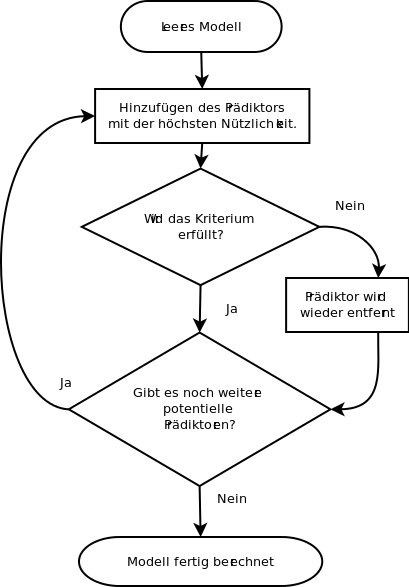
\includegraphics[width=\textwidth]{forward_stepwise.png}
	\caption{Forward Selection}
	\label{fig:forward_stepwise}
\end{figure}

In der zweiten Variante werden alle Prädikatoren in das Modell integriert und schlechte entfernt, wiederum bis das Kriterium erreicht ist. 
\begin{figure}[hb]
	\centering
	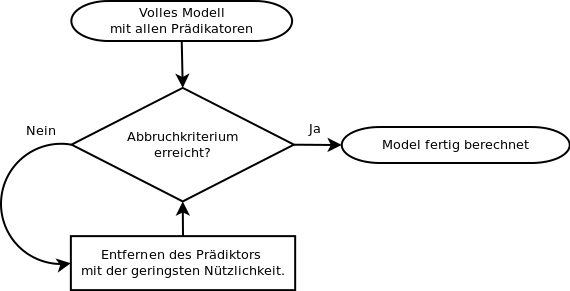
\includegraphics[width=\textwidth]{backward_stepwise.png}
	\caption{Backward Elimination}
	\label{fig:backward_stepwise}
\end{figure}

Die Aufnahme einer neuen Variable kann dazu führen, dass eine bereits im Modell vorhandene Variable obsolet wird. 
Um diesem Umstand Rechnung zu tragen werden oft forward selection und backward elimination kombiniert \cite[p. 461]{bortz2011}. 

In seltenen Fällen kann es vorkommen, dass zwei Variablen für sich das Kriterium in die Regressionsgleichung aufgenommen zu werden nicht erfüllen, jedoch zusammen zum Vorhersagepotential einen substantiellen Beitrag leisten \cite[p.261]{jacob2003applied}. 
Schrittweise Verfahren sind entsprechend nicht in der Lage solche Effekte mit zu berücksichtigen. 

Entgegen dem exhaustiven Verfahren besteht bei schrittweisen Verfahren das Problem, dass unter Umständen nicht das optimale Modell gefunden wird. 
Da die Nützlichkeitsunterschiede, welche oft nur geringe statistische Bedeutung haben, das Modell bestimmen, bezeichnet \citeA[p. 462]{bortz2011} dieses Verfahren eher zu den explorativen gehörend. 
\citeA[p. 56ff]{harrell2001regression} lehnt das Verfahren gar ab und führt ins Feld, dass sämtliche statistischen Prinzipien verletzt würden. 
\citeA{berk1978comparing} zeigte jedoch in einem Vergleich, dass die durchschnittliche Differenz der Fehlerquadratsummen zwischen exhaustiven und schrittweiser Regression kaum 7\% übertrifft. 

Zentrales Element der schrittweisen Regression ist das Mass zur Beurteilung der  Modellanpassung, welche besagt, weshalb und wann ein Modell als akzeptabel zu betrachten ist. 
Als Folge dessen wird damit auch die Anzahl relevanter Prädiktoren bestimmt.

\paragraph{Bestimmtheitsmass}  Das Quadrat des multiplen Korrelationskoeffizienten $R^2$ besagt wie viel systematische Varianz aufgeklärt wird. 
Je grösser die Zahl der unabhängigen Variablen ist, desto grösser wird das Bestimmtheitsmass, weshalb eine Korrektur vorgenommen werden muss. 
Insbesondere bei kleinem $R^2$ sollte auf Signifikanz getestet werden, entsprechend wird in schrittweisen Verfahren Prädikatoren nicht einzig aufgrund von $R^2$ selektiert. 

\paragraph{Signifikanztest} Das Verfahren wird beendet, wenn kein Prädikator mehr vorhanden ist, der das Vorhersagepotential signifikant erhöht. 
Das vergleichen zweier Regressionsgleichungen mittels Signifikanztest bedingt, dass diese geschachtelt sein müssen, das kleinere Modell muss im grösseren enthalten sein \cite[p. 508]{jacob2003applied}.

\citeA[p. 269]{derksen2011backward} diskutieren mehrere Empfehlungen für Signifikanzniveaus und weisen darauf hin, das sich über mehrere Tests der $\alpha$-Fehler kumuliert. 
In  Simulationen mit artifiziellen Daten zeigen \citeA{mundry2009stepwise} das  Problem multipler Tests beispielhaft auf. 
Daraus resultierend lehnen sie die Verwendung der schrittweisen Regression gar ab.
 
\paragraph{Informationskriterium (AIC / BIC)} Das Akaikes Informationskriterium (AIC) und Bayessche Informationskriterium (BIC) basieren auf der Maximum-Likelihood-Methode, müssen nicht geschachtelt sein und berücksichtigen die Komplexität des Modells anhand der Prädiktoranzahl. 
Die beiden Kennwerte strafen dem Prinzip der Sparsamkeit entsprechend Komplexität, was der Überanpassung entgegen wirkt.

\section{Überanpassung - Was zusammenhängt gehört rein, was einigermassen unbedeutend ist raus}\label{sparsamkeit}
\section{Zusammenfassung / Diskussion}


\blindtext

\newpage
\bibliographystyle{apacite} 
\bibliography{literature}
\newpage
\section{Anhang}
\blindtext
\newpage
\section{Selbstständigkeitserklärung}
\blindtext
\begin{comment}

\\
\\
Name: Markus Graf\\
Matriculation number:  08-91271-9\\
\\
\\
\\
\\
\\
\\
............................................................................\\
Zürich, \today
\end{comment}


\end{document}
